\section{Hybrid Workflow Behavior}
\label{sec:hybrid-workflow-behavior}

Many near term quantum applications are realized not as single shot quantum programs, but as \emph{iterative hybrid quantum classical workflows}. Representative examples include the Variational Quantum Eigensolver (VQE), the Quantum Approximate Optimization Algorithm (QAOA), and hybrid calibration and tuning routines deployed in contemporary quantum cloud environments.

To isolate the impact of hybrid workflow structure on system behavior, we conduct a controlled experiment in which physical resources, circuit characteristics, and workload composition are held constant, while only the number of quantum classical iterations per job is varied.

\begin{table}[t]
\centering
\caption{Simulation Configuration and Workload Characteristics for hybrid workflow behavior.}
\label{tab:use-case-2-summary}
\begin{tabular}{p{0.31\linewidth} p{0.60\linewidth}}
\hline
\textbf{Category} & \textbf{Configuration} \\
\hline
Workload size & 3,000 synthesis jobs  \\

Quantum workload parameters &
\begin{tabular}[t]{@{}l@{}}
Number of qubits: 10 to 20 \\
Circuit depth: 10 to 20 \\
Shots per job: 2,000 to 9,000 \\
Arrival process: Exponential ($\lambda \approx 1.04$)
\end{tabular} \\

Classical workload parameters &
\begin{tabular}[t]{@{}l@{}}
CPU units: 7 to 10 (qubit scaled) \\
Memory BW units: 14 to 20 (qubit scaled)
\end{tabular} \\

Quantum resources &
\begin{tabular}[t]{@{}l@{}}
2 $\times$ QPUs \\
IBM\_Strasbourg (127 qubits) \\
IBM\_Brussels (127 qubits)
\end{tabular} \\

Classical resources &
\begin{tabular}[t]{@{}l@{}}
2 $\times$ CPU nodes \\
8 cores, 16 threads per node \\
Base / boost: 3.8 / 5.0 GHz \\
Memory bandwidth: 51.2 GB/s
\end{tabular} \\

Resource abstraction &
\begin{tabular}[t]{@{}l@{}}
CPU capacity = threads $\times$ cpu units \\
Mem BW capacity = GB/s $\times$ mem units
\end{tabular} \\

Energy pricing & \$0.18 per kWh \\

QPU power model &
\begin{tabular}[t]{@{}l@{}}
Static power draw \\
QPU 1: 70 kW \\
QPU 2: 60 kW
\end{tabular} \\

CPU power model &
\begin{tabular}[t]{@{}l@{}}
Affine utilization based model \\
CPU 1 peak: 5.0 kW \\
CPU 2 peak: 6.5 kW
\end{tabular} \\

\hline
\end{tabular}
\end{table}

The experimental setup is listed in Table~\ref{tab:use-case-2-summary}. We use a fixed set of 3,000 synthesized quantum jobs generated with identical distributions for qubit counts, circuit depth, shot count, and classical resource requirements. The hybrid environment consists of two QPUs and two CPU devices, operated under the same scheduling policy and cost model parameters across all experimental runs.

The sole parameter that differs between experiments is the required number of hybrid iterations per job. Specifically, we evaluate seven workflow configurations with iteration counts ranging from 3 to 21 in increments of 3. Each configuration is provided as a separate workload trace. The purpose is to assure that any observed differences in execution time, energy consumption, or cost are attributable exclusively to changes in workflow structure rather than hardware variability or workload diversity.

\subsection{Iteration Scaling and the Onset of Quantum Congestion}
\label{sec:iteration-scaling}

Variational algorithms (e.g., VQE, QAOA) iteratively alternate between $k$ circuit execution rounds and classical parameter updates. Standard hybrid cloud cost models assume a linear multiplier where $k$ iterations cost $k\times$ a single iteration; the assumption holds only for the computation itself. Beyond a critical iteration count, the time a job occupies a QPU per iteration escalates by more than an order of magnitude while its computation, and the classical phase, scale perfectly linearly. This effect stems from contention across a finite quantum fleet rather than from the application; it is invisible to models that ignore device occupancy and misattributed by those that bill the occupied window as computation.


\subsection{Experimental Design}
\label{sec:iter-setup}

The experiment is a single factor sweep. We generate one batch of $N=3000$ synthetic variational jobs and replicate it seven times, altering exactly one field, namely the requested iteration count $k \in \{3,6,9,12,15,18,21\}$. Every other job attribute is bit identical across the seven traces: qubit width, circuit depth, shot count, priority, arrival timestamp, CPU core demand, and memory bandwidth demand. Any difference in the measured outcome is therefore attributable to $k$ alone, with no confounding from workload composition or arrival pattern.

Jobs request $10$ to $20$ qubits (mean $15.15$), circuit depth $10$ to $20$, $2000$ to $9000$ shots (mean $5501$), $7$ to $10$ CPU units, and $14$ to $20$ memory bandwidth units. Arrivals are replayed over a window of $2884.8$ simulation seconds, a mean rate $\lambda \approx 1.04$ jobs per second. The classical columns are not consulted: every CPU phase is admitted against a fixed budget of $8$ CPU and $20$ memory bandwidth units and runs on a CPU unit allocation drawn uniformly from $4$ to $16$, the sweep's sole stochastic element.

The target platform is a fixed hybrid inventory: two superconducting QPUs modeled on IBM Eagle r3 devices (\texttt{IBM\_Strasbourg} as QPU 1 and \texttt{IBM\_Brussels} as QPU 2, $127$ physical qubits each on the heavy hex coupling map, with their published CLOPS, quantum volume, and $T_1/T_2$ figures), and two \texttt{AMDRyzen} classical nodes, instantiated afresh for every run so that no qubit occupancy or topology state leaks between configurations. Energy is attributed per phase from constant device draws of \qty{70}{\kilo\watt} (QPU 1), \qty{60}{\kilo\watt} (QPU 2), \qty{5.0}{\kilo\watt} (CPU 1), and \qty{6.5}{\kilo\watt} (CPU 2) at $\$0.18$ per \unit{\kilo\watt\hour}. Each configuration runs to completion and is summarized over all $3000$ jobs.

Two structural features of the platform matter for what follows. First, a QPU admits several jobs concurrently, bounded not by a job slot count but by free qubits: at a mean width of $15.15$ qubits, the $254$ qubit fleet could in principle host $C \approx 16.8$ jobs at once. Second, admission is resolved at two levels, specifically aggregate qubit capacity \emph{and} physical connectivity. A job is admitted only when a \emph{connected} subgraph of free qubits exists, so the achievable concurrency is strictly below $C$ whenever the free qubits are scattered across the coupling graph.

It is convenient to summarize the concurrency demand by the dimensionless ratio
\begin{equation}
  \rho(k) \;=\; \frac{\lambda \, s_1 \, k}{C},
  \label{eq:rho}
\end{equation}
where $s_1 = \qty{0.971}{\second}$ is the QPU computation time of a single iteration, identical at every sweep point. Equation~\eqref{eq:rho} is the fraction of nominal fleet concurrency that the workload demands; it rises from $\rho = 0.18$ at $k=3$ to $\rho = 1.26$ at $k=21$ and passes unity at $k \approx 16.6$.

\subsection{Metrics and Figure Construction}
\label{sec:iter-metrics}

For each QPU phase the device records its \emph{computation} time $T_{\mathrm{comp}}$, the circuit execution time of Eq.~\eqref{eq:qpu-time}, while the broker stamps its \emph{occupancy} $T_{\mathrm{occ}}$, the window from admission at the capacity gate to release, throughout which the job is resident on a powered device; they differ by the time spent retrying the connectivity check of Section~\ref{sec:arch-qpu}, once per second, until a connected free region exists. Per job energy is charged on $T_{\mathrm{comp}}$ alone; it is the QPU phase duration entering Eq.~\eqref{eq:energy}. Since Eq.~\eqref{eq:qpu-time} depends only on job attributes, $\sum T_{\mathrm{comp}}$ is linear in $k$ \emph{by construction}: a control, not a finding. Figure~\ref{fig:iteration-knee} therefore reports three \emph{derived}, scale free views of the sweep, each chosen so that the linear scaling null hypothesis appears as a flat line and departure from linearity as departure from flatness.

\paragraph{Panel (a): computation and occupancy per iteration.}
We divide the mean per job QPU computation, QPU occupancy, and CPU phase time by $k$, the average cost of one iteration on each resource class. Under the multiplier assumption all three series are horizontal. All three share one logarithmic axis (\unit{\second} per iteration) because occupancy spans a factor of $41$ while the other two do not move.

\paragraph{Panel (b): compute fraction of occupied QPU time.}
For each run we form the ratio of sums
\begingroup
\small
\begin{equation}
  \eta \;=\; \frac{\sum T_{\mathrm{comp}}}{\sum T_{\mathrm{occ}}} \;\in\; (0, 1],
  \label{eq:eta}
\end{equation}
\endgroup
the fraction of reserved, powered QPU time that performs computation. $\eta = 1$ is exactly the multiplier assumption and serves as the reference; a second line at $\eta = \tfrac12$ marks the point past which most occupied QPU time is idle.

\paragraph{Panel (c): dispersion and tail weight.}
We plot two dimensionless descriptors of the per job turnaround distribution \emph{within} each run: the coefficient of variation $\mathrm{CV} = \sigma/\mu$, and the tail ratio $p_{95}/\mathrm{median}$. Both are invariant to the overall time scale, so they isolate changes in the \emph{shape} of the distribution from changes in its magnitude. The reference line at $\mathrm{CV}=1$ marks exponential like dispersion, the canonical signature of a queue that has begun to build.

In all three panels a shaded band marks the congested regime, its left edge where $\eta$ falls through one half, interpolated inside the $12 \to 15$ bracket ($k \approx 13$). The figure is generated from the sweep summary by \texttt{plot\_iteration\_knee.py} without smoothing or fitting.


\begin{figure*}[t]
  \centering
  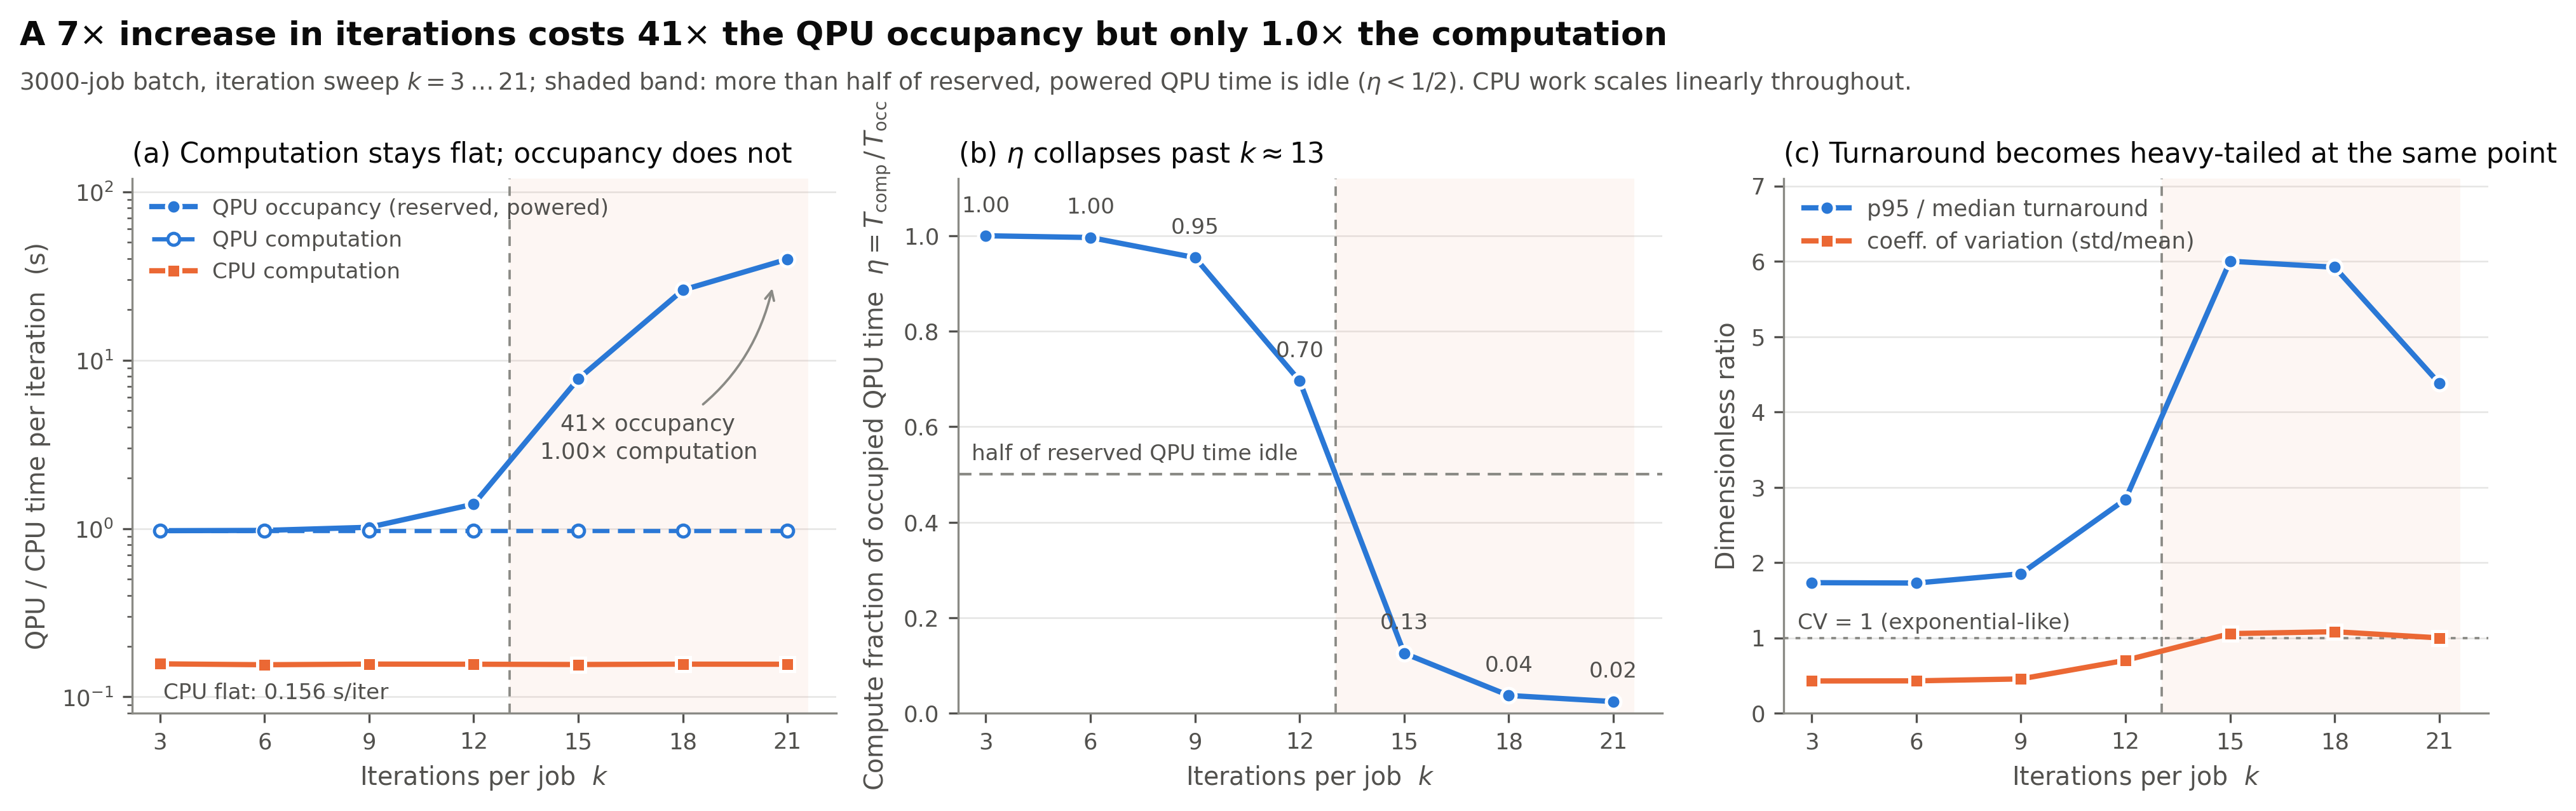
\includegraphics[width=\textwidth]{Images/Performance/plot_iteration_knee.png}
  \caption{Iteration scaling of a fixed $3000$ job variational workload on a two QPU, two CPU fleet; only $k$ varies across the seven runs. (a)~QPU time per iteration: computation is constant at \qty{0.971}{\second} while occupancy rises $41\times$; the classical phase is flat at \qty{0.156}{\second} to within $1\%$. (b)~Compute fraction of occupied QPU time, $\eta$ of Eq.~\eqref{eq:eta}; it falls through one half near $k \approx 13$ and reaches $0.024$ at $k=21$. (c)~The coefficient of variation crosses unity and the $p_{95}$/median ratio more than triples in the same bracket. The shaded band marks $\eta < \tfrac12$.}
  \label{fig:iteration-knee}
\end{figure*}

\begin{table}[t]
\centering
\caption{Iteration sweep over an identical $3000$ job trace. $\rho$ is the concurrency demand of Eq.~\eqref{eq:rho}, per iteration columns are mean phase time divided by $k$, $\eta$ is the compute fraction of Eq.~\eqref{eq:eta}, and $E$ is mean per job attributable energy. Rows below the rule lie in the shaded band.}
\label{tab:iteration-sweep}
\small
\setlength{\tabcolsep}{3.5pt}
\begin{tabular}{@{}rrrrrrrrr@{}}
\toprule
 & & \multicolumn{3}{c}{Per iteration (\unit{\second})}
 & & & \multicolumn{2}{c}{Turnaround} \\
\cmidrule(lr){3-5}\cmidrule(lr){8-9}
$k$ & $\rho$ & $T_{\mathrm{comp}}$ & $T_{\mathrm{occ}}$ & CPU & $\eta$ & $E$ (\unit{\kilo\watt\hour})
 & CV & $p_{95}/\tilde{x}$ \\
\midrule
 3 & 0.18 & 0.971 &  0.971 & 0.157 & 1.000 & 0.053 & 0.43 & 1.73 \\
 6 & 0.36 & 0.971 &  0.974 & 0.155 & 0.996 & 0.107 & 0.43 & 1.73 \\
 9 & 0.54 & 0.971 &  1.017 & 0.157 & 0.954 & 0.160 & 0.46 & 1.85 \\
12 & 0.72 & 0.971 &  1.394 & 0.156 & 0.696 & 0.213 & 0.70 & 2.84 \\
\midrule
15 & 0.90 & 0.971 &  7.727 & 0.156 & 0.126 & 0.267 & 1.06 & 6.00 \\
18 & 1.08 & 0.971 & 26.09  & 0.156 & 0.037 & 0.320 & 1.08 & 5.92 \\
21 & 1.26 & 0.971 & 39.73  & 0.156 & 0.024 & 0.373 & 1.00 & 4.38 \\
\bottomrule
\end{tabular}
\end{table}

\subsection{Results}
\label{sec:iter-results}

\paragraph{Computation is a control, and it stays flat.}
The most useful columns of Table~\ref{tab:iteration-sweep} are the two that do not move. QPU computation per iteration is \qty{0.971}{\second} at every $k$, and the measured classical phase is \qty{0.157}{\second} per iteration at $k=3$ and \qty{0.156}{\second} at $k=21$, constant to within $1\%$ across a sevenfold increase in loop length. Per job attributable energy follows, growing from $0.053$ to \qty{0.373}{\kilo\watt\hour}, a factor of $6.99$ for $7\times$ the iterations, with a QPU share flat at $98.4\%$. This is correct linear scaling measured on the same runs, which forecloses a harness artifact as the explanation for what follows.

\paragraph{The marginal iteration stops taking the same time.}
Through $k=9$ occupancy also behaves as the multiplier assumption predicts: a job holds the QPU for $0.971$, $0.974$, and \qty{1.017}{\second} per iteration. Then it breaks. Occupancy per iteration rises to $1.39$ at $k=12$, $7.73$ at $k=15$, $26.1$ at $k=18$, and \qty{39.7}{\second} at $k=21$: a $41\times$ increase in the time a job is resident on a powered QPU per iteration against a $1.00\times$ change in the time it computes there. A $21$ iteration job receives $21$ iterations that each take far longer, because the fleet is congested by jobs like itself.

\paragraph{The compute fraction collapses near $k \approx 13$.}
$\eta$ is $0.9999$ at $k=3$, $0.954$ at $k=9$, $0.696$ at $k=12$, $0.126$ at $k=15$, and $0.024$ at $k=21$, falling through one half at $k \approx 13$. Past that knee more than half, and by $k=18$ more than $96\%$, of the time a job spends resident on a cryogenically powered device is spent not computing: mean idle time per job is \qty{5.1}{\second} at $k=12$, \qty{101}{\second} at $k=15$, and \qty{814}{\second} at $k=21$, against \qty{20.4}{\second} of QPU computation. The time to drain the batch rises from \qty{2888}{\second} to \qty{4049}{\second}, and cumulative qubit utilization from $16\%$ to $89\%$.

\paragraph{Predictability collapses at the same point.}
Panel~(c) confirms this from a quantity the first two panels never touch, the shape of the turnaround distribution. Through $k=9$ turnaround is tight, with $\mathrm{CV} \le 0.46$ and a $p_{95}$ at most $1.85\times$ the median. The tail ratio reaches $2.84$ at $k=12$ and $6.00$ at $k=15$, and the CV crosses $1$ in the same bracket. The ratio narrows again at $k=21$ ($4.38$) not because the tail shortens but because the bulk has joined it: from $k=18$ to $k=21$ the median more than doubles ($267$ to \qty{574}{\second}) while the $95$th percentile grows $1.6\times$. A $k=21$ job needs \qty{23.7}{\second} of computation and waits a median of \qty{574}{\second} for it. Two quantities from different columns of the record change character in the same interval: the evidence that one mechanism is responsible.

\paragraph{The mechanism is occupancy, not work.}
Because computation is fixed, the collapse must originate in re-acquisition: a job releases its qubit region at the end of every QPU phase and re-acquires one at the next. Raising $k$ does not raise the work per iteration; it raises how long the job \emph{resides} in the system, and by Little's law a $k$ fold longer residency puts $k$ fold more jobs on the fleet at once. Concurrency demand reaches $\rho = 1$ only at $k \approx 16.6$ (Table~\ref{tab:iteration-sweep}), yet the compute fraction halves at $\rho \approx 0.78$: the knee falls while a fifth of the nominal qubit capacity is still formally free. Instrumenting the allocator shows what that gap is made of. Each blocked acquisition attempt (one second inside the phase) was classified by whether the device still held enough \emph{free} qubits for the request. At the onset of the knee, $k=12$, it did in $69.7\%$ of $14{,}963$ blocked attempts: on average $26.0$ qubits were free against $18.1$ requested, but the largest \emph{connected} free region held only $12.4$. This is connectivity fragmentation, a failure mode with no classical analogue: a heavy hex lattice that is $20\%$ free can be unable to seat an $18$ qubit circuit. As load deepens the balance shifts to plain capacity exhaustion, fragmentation accounting for $34.8\%$ of $296{,}833$ blocked attempts at $k=15$ and $14.9\%$ of $2.28$ million at $k=21$. Fragmentation initiates the collapse; saturation sustains it.

\paragraph{The energy consequence depends on what is billed.}
A superconducting QPU draws its full cryogenic baseline whenever it hosts a job, so the fleet power of Eq.~\eqref{eq:power} is paid for occupancy, computing or not. Per job energy is charged for computation only and is therefore linear in $k$: $\$0.0096$ per job at $k=3$ and $\$0.067$ at $k=21$, or $\$29$ and $\$202$ for the batch. Billing the occupied window at the same power would instead charge a $k=21$ job about $\$2.71$, roughly $1/\eta \approx 40\times$ more, and the batch about $\$8{,}100$. The difference is the cost of reserved capacity that performed no work, which under a computation based attribution falls on the facility rather than the tenant.


\subsection{Implications}
\label{sec:iter-implications}

Increasing the iteration count of a hybrid job does not make it more expensive to compute; past the knee it makes it far more expensive to \emph{hold}, and the holding dominates both the device side cost and the turnaround tail. Iteration count is therefore a \emph{capacity planning} parameter with a threshold, not a workload parameter to be optimized in isolation. An operator sizing a fleet from single job measurements at small $k$ will extrapolate linearly and under provision QPU occupancy forty fold at $k=21$, and an algorithm designer trading a longer loop for a shallower circuit may make a strictly worse system level trade even when per circuit metrics improve.


\subsection{Threats to Validity}
\label{sec:iter-validity}

Three limitations qualify these results.

First, the dispersion statistics in panel~(c) reflect variation \emph{across the $3000$ jobs within a single run} rather than replicate runs with independent random seeds. QPU computation and energy are deterministic given the trace, and an independent replicate reproduced every occupancy and dispersion statistic in Table~\ref{tab:iteration-sweep} to within $2\%$; replicate trials are still needed for confidence intervals and to resolve the knee location within the $12 \to 15$ bracket.

Second, per job energy is a sole tenant attribution: each job is charged its device's full baseline for its own computation, so per job figures cannot be summed into the facility total of Eq.~\eqref{eq:power}, and who bears the cost of idle reserved capacity is a pricing policy question the simulator exposes but does not settle.

Third, the overloaded regime ($\rho > 1$, $k \ge 18$) should be read qualitatively: turnaround there is governed by backlog drain over the finite arrival window, which is why the tail ratio recedes from $6.0$ to $4.4$ even as the median doubles. The primary result is the departure of $\eta$ from unity and its onset, not the values attained beyond it.
